\documentclass[12pt]{scrartcl}

\setlength{\parindent}{0pt}
\setlength{\parskip}{.25cm}

\usepackage{graphicx}

\usepackage{xcolor}

\definecolor{darkred}{rgb}{0.5,0,0}
\definecolor{darkgreen}{rgb}{0,0.5,0}
\usepackage{hyperref}
\hypersetup{
  letterpaper,
  colorlinks,
  linkcolor=red,
  citecolor=darkgreen,
  menucolor=darkred,
  urlcolor=blue,
  pdfpagemode=none,
  pdftitle={Lab 5.0 - Methods},
  pdfauthor={Christopher M. Bourke}
}

\definecolor{MyDarkBlue}{rgb}{0,0.08,0.45}
\definecolor{MyDarkRed}{rgb}{0.45,0.08,0}
\definecolor{MyDarkGreen}{rgb}{0.08,0.45,0.08}

\definecolor{mintedBackground}{rgb}{0.95,0.95,0.95}
\definecolor{mintedInlineBackground}{rgb}{.90,.90,1}

%\usepackage{newfloat}
\usepackage[newfloat=true]{minted}
\setminted{mathescape,
               linenos,
               autogobble,
               frame=none,
               framesep=2mm,
               framerule=0.4pt,
               %label=foo,
               xleftmargin=2em,
               xrightmargin=0em,
               startinline=true,  %PHP only, allow it to omit the PHP Tags *** with this option, variables using dollar sign in comments are treated as latex math
               numbersep=10pt, %gap between line numbers and start of line
               style=default, %syntax highlighting style, default is "default"
               			    %gallery: http://help.farbox.com/pygments.html
			    	    %list available: pygmentize -L styles
               bgcolor=mintedBackground} %prevents breaking across pages
               
\setmintedinline{bgcolor={mintedBackground}}
\setminted[text]{bgcolor={mintedBackground},linenos=false,autogobble,xleftmargin=1em}
%\setminted[php]{bgcolor=mintedBackgroundPHP} %startinline=True}
\SetupFloatingEnvironment{listing}{name=Code Sample}
\SetupFloatingEnvironment{listing}{listname=List of Code Samples}

\title{CSCE 155 - Java}
\subtitle{Lab 5.0 - Methods \& Testing}
\author{~}
\date{~}

\begin{document}

\maketitle

\section*{Prior to Lab}

Before attending this lab:
\begin{enumerate}
  \item Read and familiarize yourself with this handout.
  \item Read Chapters 5 and 29 of the \href{http://cse.unl.edu/~cbourke/ComputerScienceOne.pdf}{Computer Science I} textbook
\end{enumerate}

\section*{Peer Programming Pair-Up}

\textbf{For students in the online section:} you may complete
the lab on your own if you wish or you may team up with a partner
of your choosing, or, you may consult with a lab instructor to get
teamed up online (via Zoom).

\textbf{For students in the face-to-face section:} your
lab instructor will team you up with a partner.  

To encourage collaboration and a team environment, labs are
structured in a \emph{peer programming} setup.  At the start of
each lab, you will be randomly paired up with another student 
(conflicts such as absences will be dealt with by the lab instructor).
One of you will be designated the \emph{driver} and the other
the \emph{navigator}.  

The navigator will be responsible for reading the instructions and
telling the driver what to do next.  The driver will be in charge of the
keyboard and workstation.  Both driver and navigator are responsible
for suggesting fixes and solutions together.  Neither the navigator
nor the driver is ``in charge.''  Beyond your immediate pairing, you
are encouraged to help and interact with other pairs in the lab.

Each week you should alternate: if you were a driver last week, 
be a navigator next, etc.  Resolve any issues (you were both drivers
last week) within your pair.  Ask the lab instructor to resolve issues
only when you cannot come to a consensus.  

Because of the peer programming setup of labs, it is absolutely 
essential that you complete any pre-lab activities and familiarize
yourself with the handouts prior to coming to lab.  Failure to do
so will negatively impact your ability to collaborate and work with 
others which may mean that you will not be able to complete the
lab.  

\section{Lab Objectives \& Topics}
At the end of this lab you should be familiar with the following:
\begin{itemize}
  \item Understand how to design, document, write, and use methods in Java
  \item Design test cases and write informal unit tests
\end{itemize}

\section{Background}

Most programming languages allow you to define and use functions 
(or \emph{methods}).  Functions \emph{encapsulate} functionality into a 
unit of code that can be reused.  A function can be specified to 
take any number of inputs (called parameters or arguments) and 
return an output.  Defining and using functions has several advantages.  
First, it facilitates code reuse.  Rather than 
cutting and pasting a block of code, it can be encapsulated 
into a function and reused by calling the function anytime it needs 
to be executed.

Second, functions facilitate \emph{procedural abstraction}.  Often, 
we don't care or need to worry about the implementation 
details of a certain algorithm or procedure.  By encapsulating the 
details in a function, we only need to know how to use it (what 
inputs to provide it and what output we can expect from it).  We
don't need to worry about \emph{how} it computes its result.  For example,
up to now you've been using the standard math library's function
to compute the square root of a number $x$, but you haven't
had to worry about the details of how this computation actually
takes place.

Finally, functions naturally define a \emph{unit} of code that can
be easily tested.  Typically, unit tests are designed with 
\emph{test cases} which are input/output combinations that are
known to be correct.  Unit testing involves feeding the input to
a function and comparing the output to the \emph{expected} output.
If they match, we say the test case \emph{passes}, if not, we say
it \emph{fails}.  Unit testing gives a higher level of confidence
that our function's implementation is correct.

When defining a function, it is necessary to define its \emph{signature}.  
The signature of a function includes:
\begin{itemize}
  \item The function's identifier -- its name 
  \item The return type -- the type of variable the function returns
  \item The parameter list -- the number of parameters the function takes 
	(also called its \emph{arity}) along with their types 
\end{itemize}

\subsection{Methods in Java}

In Java, functions (usually called methods) must be declared/defined 
within a class.  This is done by declaring the method's signature and 
adding a block of code that specifies the instructions that will be executed 
when the method is invoked.  In addition, there are two modifiers that 
can be applied to methods:
\begin{itemize}
  \item \mintinline{java}{public} -- this specifies that the method is publicly 
  	visible and can be invoked by any other method.  Alternatives include 
	\mintinline{java}{private} (the method is only visible within the class) 
	and \mintinline{java}{protected} (the method is visible within the class 
	and any subclasses)
  \item \mintinline{java}{static} -- this specifies that the method belongs to the 
	class and not to instances of the class.
\end{itemize}

\section{Activities}

We have provided partially completed programs for each of the 
following activities.  Clone the lab's code from GitHub using the 
following URL: \url{https://github.com/cbourke/CSCE155-Java-Lab05}.

\subsection{Writing Methods}

Images are made up of individual \emph{pixels}.  Each pixel can be 
represented using an RGB (red-blue-green) color scheme.  RGB is 
generally used in displays and models a color with three integer 
values in the range $[0, 255]$ corresponding to the red, green and 
blue ``contribution'' to the color.  For example, the triple 
$(255, 255, 0)$ corresponds to a full red and green (additive) value
which results in yellow.  

Two common image filters are a black-and-white filter which transforms
an image into an equivalent gray-scale image, and a sepia filter which
transforms a photo to a reddish-brown monochrome to give it an old-timey
look.

We have already written a substantial program that processes an image
file and applies one of these filters.  However, you will need to write
the functions responsible for transforming an RGB value into a gray-scale
or sepia RGB value.  

To convert an RGB value to gray-scale you can use one of several
different techniques.  Each technique ``removes'' the color value by
setting all three RGB values to the same value but each technique 
does so in a slightly different way.

The first technique is to simply take the average of all three values:
  $$\frac{r + g + b}{3}$$

The second technique, known as the ``lightness'' technique averages 
the most prominent and least prominent colors:
  $$\frac{\max\{r, g, b\} + \min\{r, g, b\}}{2}$$

The luminosity technique uses a weighted average to account for a human 
perceptual preference toward green, setting all three values to:
  $$0.21 r + 0.72 g + 0.07 b$$
In all three cases, the integer values should be \emph{rounded} rather 
than truncated.

A sepia filter sets different values to each of the three RGB components 
using the following formulas.  Given a current $(r,g,b)$ value, the sepia
tone RGB value, $(r',g',b')$ would be:
$$\begin{array}{ll}
  r' &= 0.393r + 0.769g + 0.189b \\
  g' &= 0.349r + 0.686g + 0.168b \\
  b' &= 0.272r + 0.534g + 0.131b
\end{array}$$
As with the gray-scale techniques, values should be rounded.  Moreover, if
any of the values exceeds 255, they should be reset to 255 to stay within
the valid RGB color range.

\subsubsection*{Instructions}

In this exercise, you will design and write a ``color utilities'' 
library by implementing the methods described below.  We've provided 
a class, \mintinline{java}{ColorUtils} with a few methods already
completed for you.  You'll place your methods in the same class.

\begin{itemize}

  \item Run the \mintinline{java}{ColorUtilsTester} file which 
  contains several informal unit tests for the methods in 
  \mintinline{java}{ColorUtils}.  Observe that one of the tests
  will fail.  Fix the \mintinline{java}{toGrayScaleAverage} method so 
  that it passes the test.  Use this as an opportunity to observe:
  \begin{itemize}
    \item How to use the \mintinline{java}{RGB} class 
    \item How methods are defined in Java
    \item How methods are documented in Java
  \end{itemize}
  
  Be sure to write doc-style documentation for all of
  the following methods.
  
  \item Write a helper method that returns the \emph{minimum}
  of 3 integers.  Name your function \mintinline{java}{min}.

  \item Write a method that takes an \mintinline{java}{RGB} value and
  uses the lightness technique to return the gray-scale 
  \mintinline{java}{RGB} value.  
  Name your method \mintinline{java}{toGrayScaleLightness}

  \item Write a method that takes an \mintinline{java}{RGB} value and
  uses the luminosity technique to return the gray-scale 
  \mintinline{java}{RGB} value.  
  Name your method \mintinline{java}{toGrayScaleLuminosity}

  \item Write a method that takes an \mintinline{java}{RGB} value and
  computes a sepia-tone \mintinline{java}{RGB} value.
  Name your method \mintinline{java}{toSepia}.
  
  \item Write doc-style documentation for all your functions.
\end{itemize}

\subsection{Ad-Hoc Testing}

We've provided an application interface (see \mintinline{java}{ImageDriver}
that loads and saves images specified as \emph{command line arguments}.
\begin{itemize}
  \item You only need to specify the file names
  \item It is assumed the files are in the \mintinline{text}{images}
  \item The output file will be in the same directory, you may need to
  \emph{refresh} your project in Eclipse if they do not show up automatically
\end{itemize}
The program uses your methods to convert the image and save it to a new file.

Do some \emph{ad-hoc testing} using this application: convert the
images provided as part of the project and view the results.  You 
can also try converting some of your own images.  If your functions
are correct, the image conversion should look something like 
Figure \ref{fig:imageComparisons}.

\begin{figure}[h]
\centering
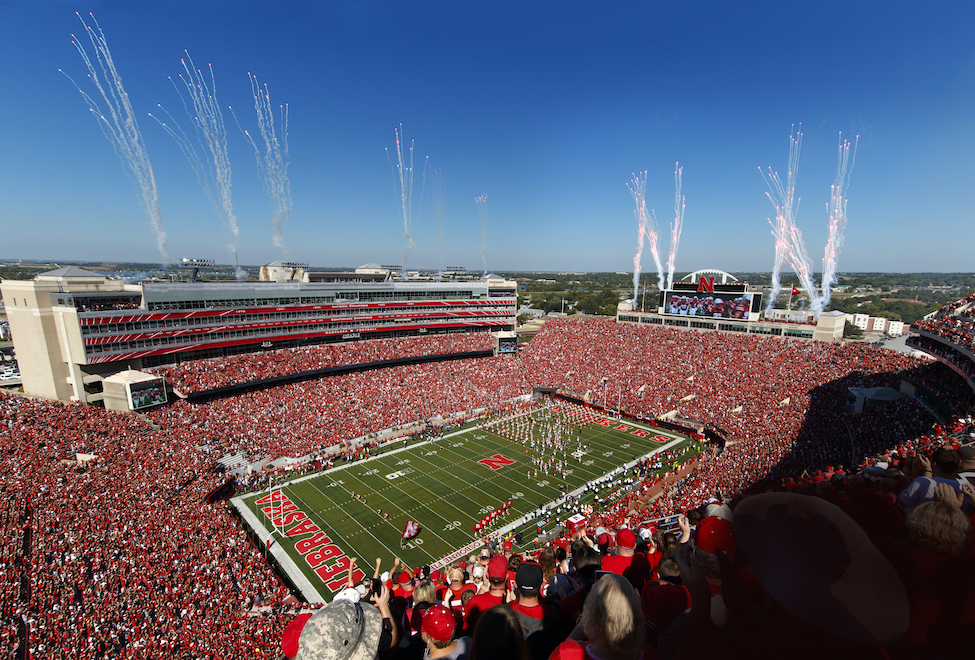
\includegraphics[scale=0.20]{../images/memorialStadium}
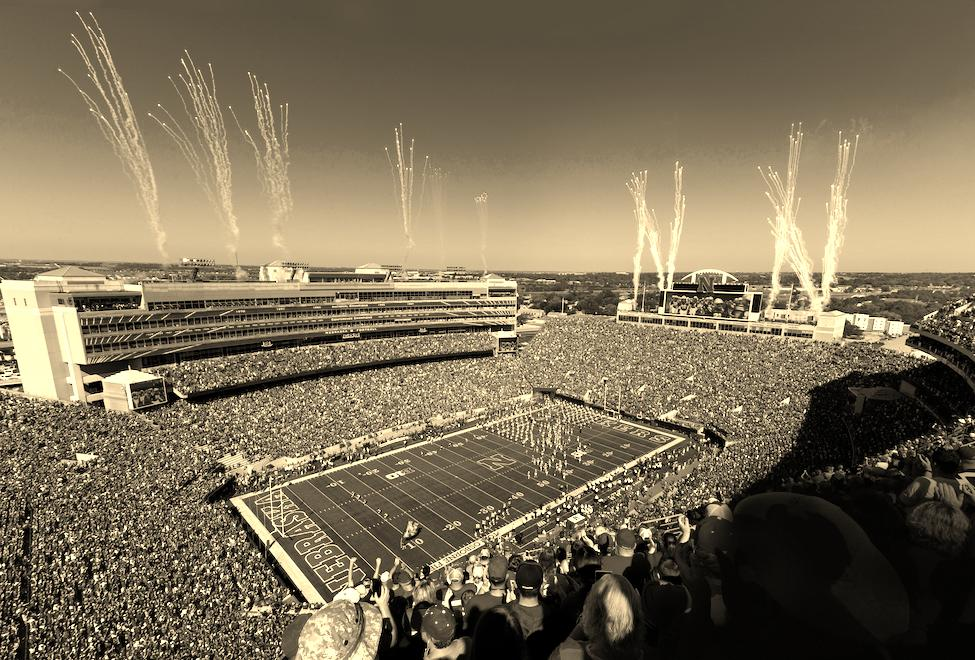
\includegraphics[scale=0.20]{../images/memorialStadiumSepia}
\caption{Memorial Stadium.  Original image (left) and Sepia-toned image (right).}
\label{fig:imageComparisons}
\end{figure}

\subsection{Writing Tests}

Testing is a fundamental step in software development.  The most common types
of tests are \emph{unit tests} and the most common ``unit'' is a function.
You may have already ``tested'' your functions by running the project and 
viewing the resulting images.  However, for your final activity, you will
write (informal) \emph{automated} unit tests to test your functions more 
rigorously.  

Some starter unit testing code has already been provided in 
\mintinline{java}{ColorUtilsTester}.  Each block of code calls a function
with some inputs and compares the return value to the \emph{expected}
output.  If they match, the test passes, if not it fails.  A message is
printed to the user and the total number of passed/failed test cases is
reported.  

Using this starter code as an example, add more test cases for the 
other functions.  You should write at least 1 test case for 
\emph{each} function you wrote.  

\section{Handin/Grader Instructions}

\begin{enumerate}
  \item Hand in your completed files:
  \begin{itemize}
    \item \mintinline{text}{ColorUtils.java}
    \item \mintinline{text}{ColorUtilsTester.java}
  \end{itemize}
  through the webhandin (\url{https://cse-apps.unl.edu/handin}) 
  using your cse login and password.  
  \item Even if you worked with a partner, you \emph{both} should
  turn in all files.
  \item Verify your program by grading yourself through the
  webgrader (\url{https://cse.unl.edu/~cse155h/grade/}) using the
  same credentials.
\end{enumerate}



\end{document}
